\documentclass[12pt]{article}
\usepackage{amsmath,amssymb}
\usepackage{geometry}
\geometry{margin=1in}
\usepackage[hidelinks]{hyperref}
\setlength{\parindent}{0pt}
\usepackage{xcolor}
\usepackage{etoolbox}  %Supports toggle commands
\definecolor{darkblue}{RGB}{0,0,139}
\usepackage{graphicx}

%SETTINGS
\newtoggle{solutions} \togglefalse{solutions}

\begin{document}

\begin{center}
\textbf{Problem Set 1} \\
Introduction to Health Economics: EC 387 \\
Boston University \\
Spring 2026 \\
Professor Pauline Mourot
\end{center}



\noindent \textbf{Exercise 1: Useful review mathematics \& microeconomics}\\


\noindent \textbf{I.} Solve for $P$ and $Q$ in the following two-equation systems:

\noindent \textbf{a.}
\begin{align*}
&Q = 30 + 5P\\
&Q = 100 - 5P
\end{align*}

\iftoggle{solutions}{
{\color{darkblue}
Since both equations are already in terms of $Q$,
the simplest way to solve these kinds of problems is to set the equations equal to each other,
and then use algebra to solve for $P$:

\begin{align*}
30 + 5P &= 100 - 5P \\
10P &= 70 \\
P &= 7
\end{align*}

\begin{equation*}
Q = 30 + 5(7) = 65
\end{equation*}

}}{}

\noindent \textbf{b.}
\begin{align*}
&Q = 5 + (0.5)P\\
&Q = 47 - 10P
\end{align*}

\iftoggle{solutions}{
{\color{darkblue}
\begin{align*}
5 + 0.5P &= 47 - 10P \\
10.5P &= 42 \\
P &= 4
\end{align*}

\begin{equation*}
Q = 5 + 0.5(4) = 7
\end{equation*}
}}{}

\noindent \textbf{II.}. Take the derivative of the following equations with respect to $P$ (that is, solve for $\frac{\partial Q}{\partial P}$):

\noindent \textbf{a.} $Q = 30 - \frac{P}{6}$

\iftoggle{solutions}{
{\color{darkblue}
The general formula for calculating derivatives of polynomials is the following
(where $a,b,c$ are constants):

\begin{equation*}
Q = aP^b + c
\end{equation*}

\begin{equation*}
\frac{\partial Q}{\partial P} = abP^{b-1}
\end{equation*}

Note that this formula holds for non-integer exponents, as well.
Also, note that $aP^0 = a$ and $aP^1 = aP$.
Using the formula above gives following expression:

\begin{align*}
Q &= 30 - \frac{1}{6} P^1\\
\frac{\partial Q}{\partial P} &= -\frac{1}{6}P^{1-1} = -\frac{1}{6}P^{0}= -\frac{1}{6}
\end{align*}
}}{}

\noindent \textbf{b.} $Q = P^2 + 10P - 8$

\iftoggle{solutions}{
{\color{darkblue}
\begin{align*}
Q &= P^2 + 10P - 8 \\
\frac{\partial Q}{\partial P} &= 2P + 10
\end{align*}
}}{}

\noindent \textbf{c.} $Q = 3P^3 - 20P + 1000000$

\iftoggle{solutions}{
{\color{darkblue}
\begin{align*}
Q &= 3P^3 - 20P + 1000000 \\
\frac{\partial Q}{\partial P} &= 9P^2 - 20
\end{align*}
}}{}

\vspace{7mm}
\noindent \textbf{III.} For each of the equations below, report the partial derivative of $Y$ with respect to $K$ and $L$ (that is, solve for $\frac{\partial Y}{\partial K}$ and $\frac{\partial Y}{\partial L}$):

\noindent \textbf{a.} $Y = K^{1/2}L^{1/2}$

\iftoggle{solutions}{
{\color{darkblue}
\begin{align*}
\frac{\partial Y}{\partial K} &= \frac{1}{2}K^{-1/2}L^{1/2} \\
\frac{\partial Y}{\partial L} &= \frac{1}{2}K^{1/2}L^{-1/2}
\end{align*}
}}{}

\noindent \textbf{b.} $Y = K^2 L^3$

\iftoggle{solutions}{
{\color{darkblue}
\begin{align*}
\frac{\partial Y}{\partial K} &= 2K L^3 \\
\frac{\partial Y}{\partial L} &= 3L^2 K^2
\end{align*}
}}{}

\noindent \textbf{c.} $Y = K^{1/3}L^{2/3}$

\iftoggle{solutions}{
{\color{darkblue}
\begin{align*}
\frac{\partial Y}{\partial K} &= \frac{1}{3}K^{-2/3}L^{2/3} \\
\frac{\partial Y}{\partial L} &= \frac{2}{3}K^{1/3}L^{-1/3}
\end{align*}
}}{}

\vspace{7mm}
\noindent \textbf{IV.} Find the value of $P$ which maximizes the following function (and the value of $Y$ at the maximum):

\noindent \textbf{a.} $Y = 100 P - 5P^2$

\iftoggle{solutions}{
{\color{darkblue}
\begin{align*}
\frac{\partial Y}{\partial P} &= 100 - 10P = 0 \\
P^* &= 10
\end{align*}

\begin{equation*}
Y^* = 100*10 - 5(10)^2 = 500
\end{equation*}
}}{}

\noindent \textbf{b.} $Y = 47 P - 10P^2$

\iftoggle{solutions}{
{\color{darkblue}
\begin{align*}
\frac{\partial Y}{\partial P} &= 47 - 20P = 0 \\
P^* &= 2.35
\end{align*}

\begin{equation*}
Y^* = 47*2.35 - 10(2.35)^2 = 55.225
\end{equation*}
}}{}

\vspace{7mm}
\noindent \textbf{V.} Find the value of $Q$ which minimizes the following function
(and the value of $Y$ at the minimum):

\noindent \textbf{a.} $Y = Q^2 + 30Q - 10$

\iftoggle{solutions}{
{\color{darkblue}
\begin{align*}
\frac{\partial Y}{\partial Q} &= 2Q + 30 = 0 \\
Q^* &= -15
\end{align*}

\begin{equation*}
Y^* = (-15)^2 + 30(-15) - 10 = -235
\end{equation*}
}}{}

\noindent \textbf{b.} $Y = 50 + 0.5 Q^2 - 7.5Q$

\iftoggle{solutions}{
{\color{darkblue}
\begin{align*}
\frac{\partial Y}{\partial Q} &= Q -7.5 = 0 \\
Q^* &= 7.5
\end{align*}

\begin{equation*}
Y^* = 50(7.5) + 0.5(7.5)^2 - 7.5(7.5) = 21.875
\end{equation*}
}}{}

\medskip

\noindent \textbf{VI.}. A monopolist faces a demand curve of $Q = 100 - P$ and cost function $C(Q) = 10 + 5Q$.

\noindent \textbf{a.} What is the revenue of the firm as a function of $Q$?

\iftoggle{solutions}{
{\color{darkblue}
To find revenue, we simply re-arrange the demand curve to solve for $P$ and substitute into the formula for revenue:

\begin{align*}
R &= PQ \\
P &= 100 - Q \\
R &= (100 - Q)Q = 100Q - Q^2
\end{align*}
}}{}

\noindent \textbf{b}. What is the marginal revenue curve of the firm?

\iftoggle{solutions}{
{\color{darkblue}
Marginal revenue is simply the derivative of revenue function with respect to $Q$:

\begin{equation*}
MR = \frac{\partial R}{\partial Q} = 100 - 2Q
\end{equation*}
}}{}

\noindent \textbf{c}. What is the profit-maximizing price and quantity for the monopolist to charge?

\iftoggle{solutions}{
{\color{darkblue}
Step 1: Compute marginal revenue (MR) curve

\begin{equation*}
MR = 100 - 2Q
\end{equation*}

Step 2: Compute marginal cost (MC) curve

\begin{equation*}
MC = \frac{\partial C}{\partial Q} = 5
\end{equation*}

Step 3: Set $MR = MC$, solve for optimal $Q$

\begin{align*}
100 - 2Q &= 5 \\
Q^* &= 47.5
\end{align*}

Step 4: Use demand curve to find optimal $P$

\begin{equation*}
P^* = 100 - 47.5 = 52.5
\end{equation*}
}}{}

\noindent \textbf{d}. What is their profit at this point?

\iftoggle{solutions}{
{\color{darkblue}
\begin{align*}
PROFIT &= REVENUE - COST \\
&= (52.5)(47.5) - (10 + 5(47.5)) \\
&= 2246.25
\end{align*}
}}{}

\noindent \textbf{e}. If the monopolist raises its price, will revenue increase or decrease? Explain intuition in 1-2 sentences.

\iftoggle{solutions}{
{\color{darkblue}
A profit-maximizing monopolist will always operate in the elastic portion of the demand curve. Because of this, if the monopolist were to increase prices, revenue would DECREASE. Note that this is true even if the monopolist has zero costs.
}}{}

\vspace{10mm}


\noindent \textbf{Exercise 2: Simplified Grossman model}\\

This problem works through a simplified version of the Grossman model. Individuals have the following utility function for consumption, $c$:

\begin{equation*}
U(c) = \log(c)    
\end{equation*}

where $log()$ is the natural logarithm function, as usual.

\vspace{2mm}

Consumption is purchased from labor earnings, $y$, which is product of the individual's hourly wage $w$ and total hours worked, $T_w$.\\
In other words, $c = y = w \times T_w$.

\vspace{2mm}

Total hours available is $\Theta$, and must be split between work hours $T_w$, hours spent sick $T_S$, and hours spent producing health $T_H$.
Health, $H$, is produced solely from time spent producing health (e.g., exercise); i.e., $H = T_H$.

\vspace{2mm}

Health does not affect utility directly, but it affects hours spent sick, $T_S$, which cannot then be spent either working or producing health,
as indicated by the following equation:

\begin{equation*}
T_S = \Theta \exp(-H) = \Theta \exp(-T_H)
\end{equation*}

\medskip

NOTE: The main simplifications of this model relative to the textbook Grossman model are the following:\\
(1) there is no direct consumption of healthcare, only time spent investing in good health,\\
(2) utility depends only on non-health consumption $c$, so health does not raise utility directly, and\\
(3) there is no ability for individuals to choose leisure time.\\
All time must be split between work hours, hours spent producing health, and hours spent being sick.

\medskip
\noindent\textbf{a.} Write down the total ``budget constraint'' for time.
\medskip

\iftoggle{solutions}{
{ \color{darkblue}

\begin{align*}
    &T_w + T_H = \Theta - T_S = \Theta (1 - \exp(-T_H)) \\
    \Rightarrow &\frac{T_w + T_H}{1 - \exp(-T_H)} = \Theta
\end{align*}

}}

\medskip
\noindent\textbf{b.} Derive an equation for the ``production possibility frontier'' for $H$ and $c$,
and then graph the equation for the specific case of $w = 25$ and $\Theta = 100$ (with $H$ on x-axis and $c$ on y-axis),
carefully labeling the minimum and maximum values of this function.

\medskip

\iftoggle{solutions}{
{ \color{darkblue}

The equation for the production possibility frontier for $H$ and $c$ comes from using $c = wT_w$ and $H = T_H$ and substituting $T_w$ by the solution from (a). Thus, the PPF is given by

\begin{equation*}
\frac{c + wH}{1 - e^{-H}} = w\Theta
\end{equation*}

For $w = 25$ and $\Theta = 100$, the above becomes:

\begin{equation*}
\frac{c + 25H}{1 - e^{-H}} = 25 \times 100
\end{equation*}

Use the above equation to graph in the $(c,H)$ plane.

\begin{center}
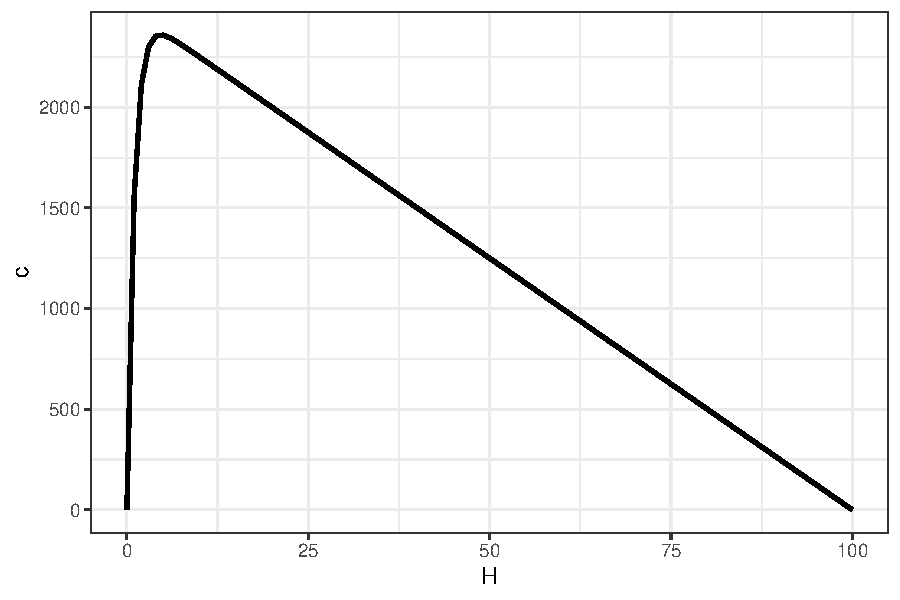
\includegraphics[width=0.6\textwidth]{./graph_ps1ex1b.pdf}
\end{center}

}}

\medskip
\noindent\textbf{c.} Solve for the optimal (utility-maximizing) choices of $T_w$, $T_H$, and $c$ (for any value of $w$ and $\Theta$).
(HINT: One can set up the problem by substituting expressions so that the only thing the consumer is choosing is amount of time spent investing in good health,
because this in turn determines time spent being sick, which then determines time spent working,
which then determines earnings and thus consumption.)

\medskip

\iftoggle{solutions}{
{ \color{darkblue}

The individual's maximization problem is:

\begin{equation*}
\max_{c,H} \log(c)
\end{equation*}

subject to the constraint in part (b).

\medskip

The above can re-written as:

\begin{equation*}
\max_H \log \left( w\Theta(1 - e^{-H}) - wH \right)
\end{equation*}

Differentiating the above and solving for $H$, we get:

\begin{equation*}
T_H = H = \log \Theta
\end{equation*}

Substitute into the constraint for $c$, and solve for work and sick time to get:

\begin{align*}
&c = w(\Theta - 1 - \log \Theta)\\
&T_w = \Theta - 1 - \log \Theta\\
&T_S = 1
\end{align*}
}}

\medskip
\noindent\textbf{d.} Now suppose that there is a tax cut that effective raises individual's after-tax wage
(so in model can treat this as increase in $w$).
What happens to time spent working? Provide an economic explanation for this in 1-3 sentences.

\medskip

\iftoggle{solutions}{
{ \color{darkblue}

The raise of wage does not have any effect on the time spent working. From part (a) and (c),
we know that the individual will spend working all his time except for when she is sick or producing health.
In this specific problem, the individual does not care about health (health does not enter the utility function directly),
so the optimal time spent producing health does not depend on wages.
Any increase in wages will just allow her to increase consumption,
which is what she cares about.
Note that even though she doesn't care about health directly, the level of health will still be positive.
This is because health increases her productive (working) time.
}}

\end{document}